\subsection{Moonpig}~\label{study-moonpig}
Moonpig is an e-commerce business in Europe that sells greeting cards and related gifts online. They have a highly rated mobile app, with overall ratings of 4.8/5 in Google Play and the Apple App Store. Their software engineering team have been actively involved in encouraging the wider software engineering community to learn and practice good software development practices, for example by hosting Coding DoJos~\footnote{Historical examples available online on twitter \url{https://mobile.twitter.com/moonpigtech} and in a \href{https://www.codurance.com/publications/newsletters/2020-02-13-newsletter}{Codurance newsletter} from February 2020, for example.}.
{\renewcommand{\arraystretch}{0.8}% Tighter
\begin{table}[htbp!]
    \centering
    \small
    \setlength{\tabcolsep}{1pt}
    \begin{tabular}{ll}
       % Question &Answer  \\
       \toprule
       Website &\url{https://www.moonpig.com/uk/} \\
       Founded &2000 \\
       Business Domain & Greeting cards and gifts \\
       Business type & e-commerce \\
       Technologies  & Native apps, Robospice, \\
       & AWS, GraphQL, nodeJS, \\
       & Commercetools, ContentStack, ... \\
       Source code  &Closed and not available for research \\
       Analytics used by team &Firebase, Google Play Console \\
       Development Practices & High performance engineering, ATDD, \\
         & micro-services architecture \\
       \midrule
       User base &100,000's for the Android app\\
       Installations &1,000,000+ for the Android app\\
       \midrule
       Research methods &In person interviews, email discussions, remote testing \\
       Analytics collected &Google Play Console with Android Vitals \\
       Research software &They used Vitals-Scraper, otherwise none applicable.\\
       Additional data collected &Interview notes and emails \\
       Active period &June 2019 `\\
       \bottomrule
    \end{tabular}
    \caption{Case Study key facts: Moonpig}
    \label{tab:moonpig_anaytics_overview}
\end{table}
}

\begin{comment}
Sources: 
- 4.8 rating in Apple App Store https://apps.apple.com/app/id393730279
- 4.8 rating in Google Play, and install count  https://play.google.com/store/apps/details?id=com.commonagency.moonpig.uk
- ATDD https://medium.com/moonpigtech/the-android-testing-approach-part-1-atdd-6e26e3851c08
- High Performance Engineering https://medium.com/moonpigtech/working-remotely-as-a-high-performance-engineering-team-at-moonpig-957b267de1d4
- micro services (in 2020) https://medium.com/moonpigtech/introducing-the-moonpig-engineering-blog-c3fde37f06bd
- Robospice - email discussions and Android Vitals crash reports
\end{comment}

\begin{figure}
    \centering
    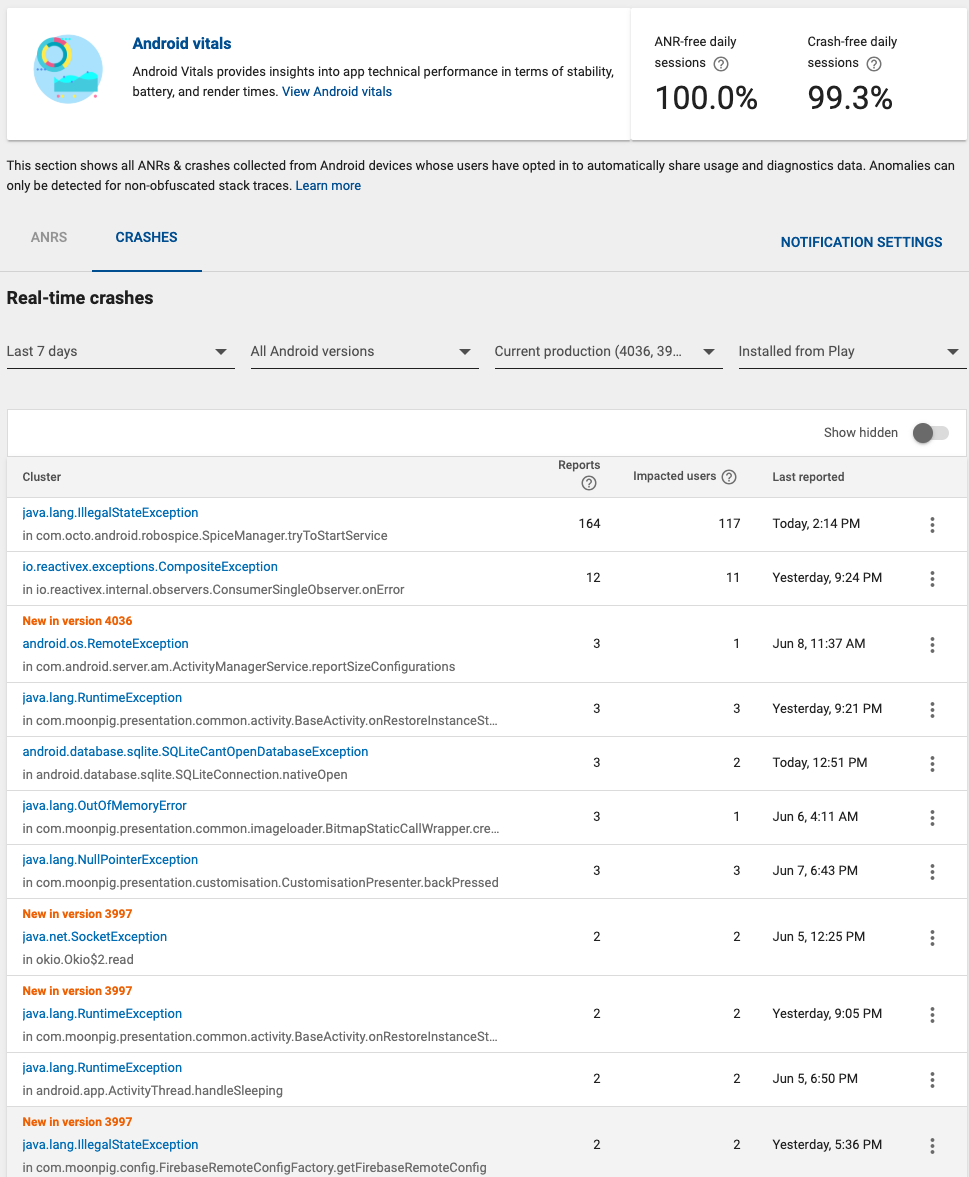
\includegraphics[width=13cm]{images/android-vitals-screenshots/moonpig/real-time-crashes-Screenshot-2019-06-10-at-15.42.34.png}
    \caption{Android Vitals: Moonpig snapshot of top crashes \nth{10} June 2019}
    \label{fig:av-moonpig-top-real-time-crashes-10-jun-2019}
\end{figure}

In Figure~\ref{fig:av-moonpig-top-real-time-crashes-10-jun-2019} Android Vitals shows the most frequent crash clusters for the production releases of the Moonpig Android app. The majority of crashes were an \texttt{IllegalStateException} in a third-party library SpiceManager, part of the RoboSpice opensource project https://github.com/stephanenicolas/robospice . 

This crash is an excellent example of how changes and new developments in the ecosystem can render what was reliable working software into software that is no longer fit for purpose, \emph{i.e.} RoboSpice was developed in 2012 to help developers simplify coding of asynchronous networking requests \url{https://github.com/stephanenicolas/robospice} and the library worked really well at the time and for several years afterwards. It became popular as a result and was used widely by many teams, including at Moonpig. However, as the Google Android platform morphed some of the changes to Android were incompatible with RoboSpice. And with Android Oreo (Release 8.0) changes to the way background services worked broke the functionality of the library sufficiently that the project was archived by the creator and project owner \url{https://github.com/stephanenicolas/robospice/issues/467} 

For apps that used RoboSpice the crash rate increased on the newer releases of Android, for example Figure~\ref{fig:av-moonpig-crash-rate-groupings} shows the crash rates by Android version were lowest on Android 7, higher for Android 8 and 8.1, and significantly higher again for Android 9. The teams needed to allocate time and energy to finding a suitable alternative to RoboSpice and then implement and test the new approach. Android Vitals helped provide an indication of the effects of the crashed and therefore provided evidence the development team could use to assess and prioritise the work.

\begin{figure}
    \centering
    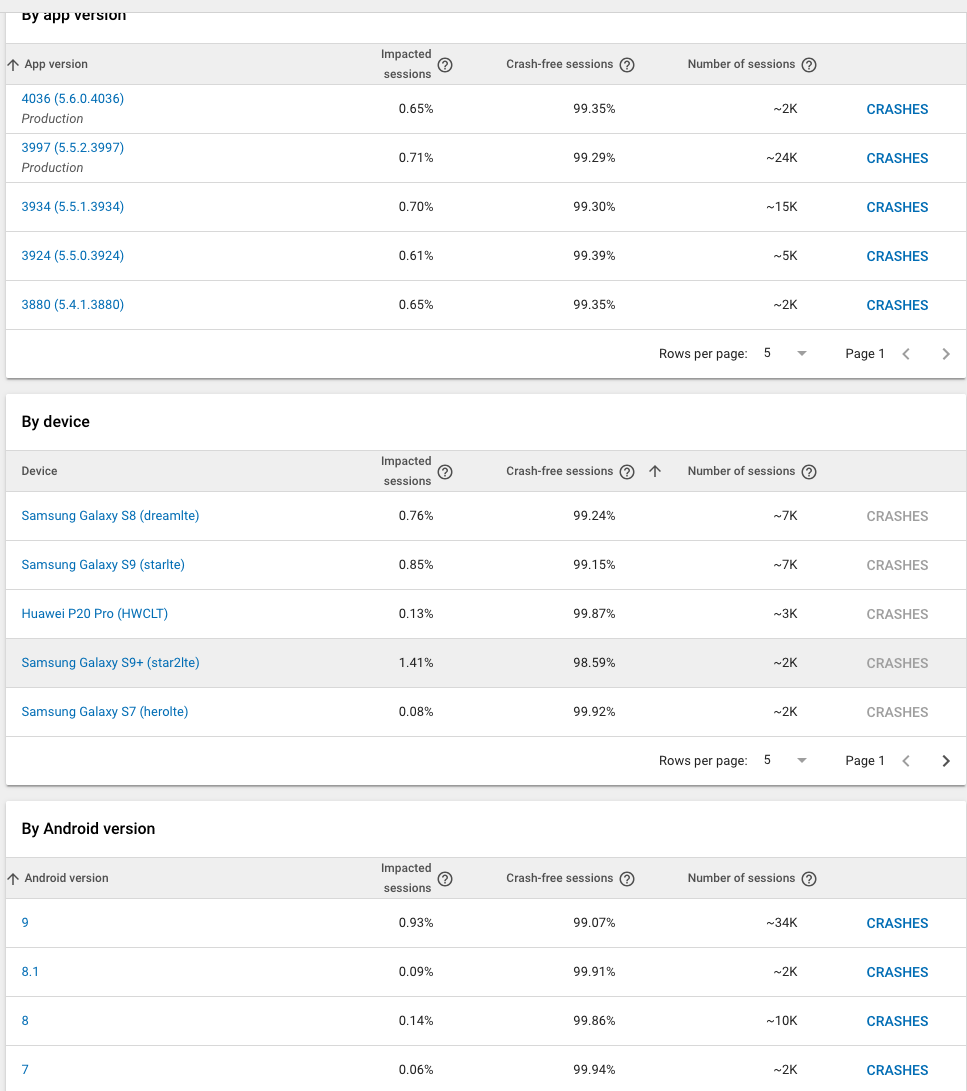
\includegraphics[width=13cm]{images/android-vitals-screenshots/moonpig/Screenshot 2019-06-10 at 15.41.23.png}
    \caption{Android Vitals: Moonpig various groupings of the crash rate \nth{10} June 2019}
    \label{fig:av-moonpig-crash-rate-groupings}
\end{figure}
